\documentclass[a4paper,11pt]{article}
\usepackage{a4wide}
\usepackage{fullpage}
\usepackage[utf8x]{inputenc}
\usepackage[slovene]{babel}
\selectlanguage{slovene}
\usepackage[toc,page]{appendix}
\usepackage[pdftex]{graphicx} % za slike
\usepackage{setspace}
\usepackage{color}
\usepackage{amsmath}
\usepackage[table]{xcolor}
\usepackage{tabularx}
\usepackage{float}
\usepackage{hhline}
\definecolor{light-gray}{gray}{0.95}
\usepackage{listings} % za vključevanje kode
\usepackage{hyperref}
\renewcommand{\baselinestretch}{1.2} % za boljšo berljivost večji razmak
\renewcommand{\arraystretch}{1.2}
\hyphenpenalty=10000
\newcolumntype{Y}{>{\centering\arraybackslash}X}
\usepackage[font=small, skip=11pt, hypcap=true]{caption}
\usepackage{indentfirst}
\setlength{\parskip}{11pt}

\title{Temperaturna plošča: serijski algoritem}
\author{Rok Grmek, Matej Klemen}
\date{\today}

\begin{document}

\maketitle

\section{Opis problema}

V okviru predmeta Porazdeljeni sistemi rešujeva problem temperaturne plošče. Na tem problemu bova tekom semestra spoznavala različne pristope za paralelno programiranje, ampak najprej potrebujeva osnovo - serijski algoritem.

Problem temperaturne plošče je predstavljen s ploščo, ki je na treh straneh (zgoraj, levo in desno) segreta na 100 °C, na spodnji stranici pa ohlajena na 0 °C. Zanima nas, kako se v takem primeru toplota porazdeli po plošči (primer porazdelitve temperature je viden na sliki \ref{primer-temperaturne-plosce}).

\begin{figure}[H]
\begin{center}

\includegraphics[scale=0.6]{primer-temperaturne-plosce.png}
\caption{Primer temperaturne plošče, kjer rdeča barva prikazuje najvišjo, temno modra barva pa najnižjo temperaturo.}
\label{primer-temperaturne-plosce}
\end{center}
\vspace{-25pt}
\end{figure}

Iskala bova stacionarno rešitev enačbe \(\nabla^2 W = f(x, y)\), pomagala pa si bova z metodo končnih diferenc. Ploščo bova najprej razdelila na mrežo točk in posameznim točkam določila začetne vrednosti. Nato bova v vsaki točki izračunala novo temperaturo na podlagi sosednjih točk. Postopek računanja novih točk se bo ponavljal, dokler rešitev ne skonvergira.

\section{Opis uporabljene metode}

\subsection{Algoritem}

Program ima dva načina delovanja. Če je nastavljena zastavica \textit{TIME\_MEASUREMENT}, se bo program za podane argumente izvedel 100-krat in izračunal nekaj uporabnih statistik. Ta način je namenjen predvsem opazovanju hitrosti izvajanja programa. Sicer pa se bo program izvedel 1-krat in na koncu vizualiziral porazdelitev temperature na plošči. V nadaljevanju je opisan slednji način izvajanja, celotno delovanje programa pa je predstavljeno tudi z diagramom zaporedja, vidnim na sliki \ref{diagram-zaporedja}.

Algoritem sprejme 3 argumente: višino plošče, širino plošče in število iteracij (v nadaljevanju označeno s \textit{k}), ki jih bo algoritem izvedel. Plošči, ki jo določata vnešena višina in širina, algoritem na vseh štirih stranicah doda pas širine 1, ki služi za nastavljanje robnega pogoja temperature. Novi dimenziji sta torej: 
\[vi\breve{s}ina := vi\breve{s}ina + 2 \quad in \quad \breve{s}irina := \breve{s}irina + 2.\]
Na začetku se alocirata dve tabeli dimenzij $ vi\breve{s}ina \times \breve{s}irina$. Ena predstavlja trenutno stanje plošče, druga pa stanje plošče v prejšnji iteraciji. Alokaciji sledi inicializacija plošče - trem stranicam (levi, desni, zgornji) algoritem nastavi temperaturo na 100 °C, eni (spodnji) pa na 0 °C. Vsem ostalim celicam plošče se zaporedno (\textit{od zgoraj navzdol, od leve proti desni}) dodeli povprečje leve sosednje, zgornje sosednje, povsem desne ter povsem spodnje celice plošče. Eno izmed plošč algoritem izbere kot ploščo trenutnega, drugo pa kot ploščo prejšnjega stanja.
\indent \par Nato sledi glavna zanka, ki se ponovi \textit{k}-krat. V vsaki iteraciji gre algoritem skozi ``dinamične'' celice plošče (celice, ki niso del katerega izmed robov plošče) in za vsako tako celico c[i][j] v \textit{i}-ti vrstici in \textit{j}-tem stolpcu po naslednji formuli izračuna novo temperaturo:
\[ c[i][j] := \frac{c'[i - 1][j] + c'[i][j - 1] + c'[i][j + 1] + c'[i + 1][j]}{4},\]
kjer $c'[i][j]$ predstavlja temperaturo celice v \textit{i}-ti vrstici in \textit{j}-tem stolpcu v prejšnji iteraciji. Ob vsakem izračunu nove temperature algoritem izračuna še absolutno razliko med trenutno (novo) in prejšnjo temperaturo ter jo v primeru, da je to v trenutni iteraciji največja izračunana absolutna razlika temperatur, shrani. Ob koncu iteracije algoritem zamenja vlogi plošč - tista, ki je do sedaj predstavljala prejšnje stanje plošče, bo v naslednji iteraciji vsebovala novo stanje plošče in obratno.

Na koncu algoritem izpiše največjo absolutno razliko temperatur in zažene vizualizacijo končnega stanja temperaturne plošče. O vizualizaciji temperaturne plošče pa je več napisano v naslednjem poglavju.

\begin{figure}[H]
\begin{center}
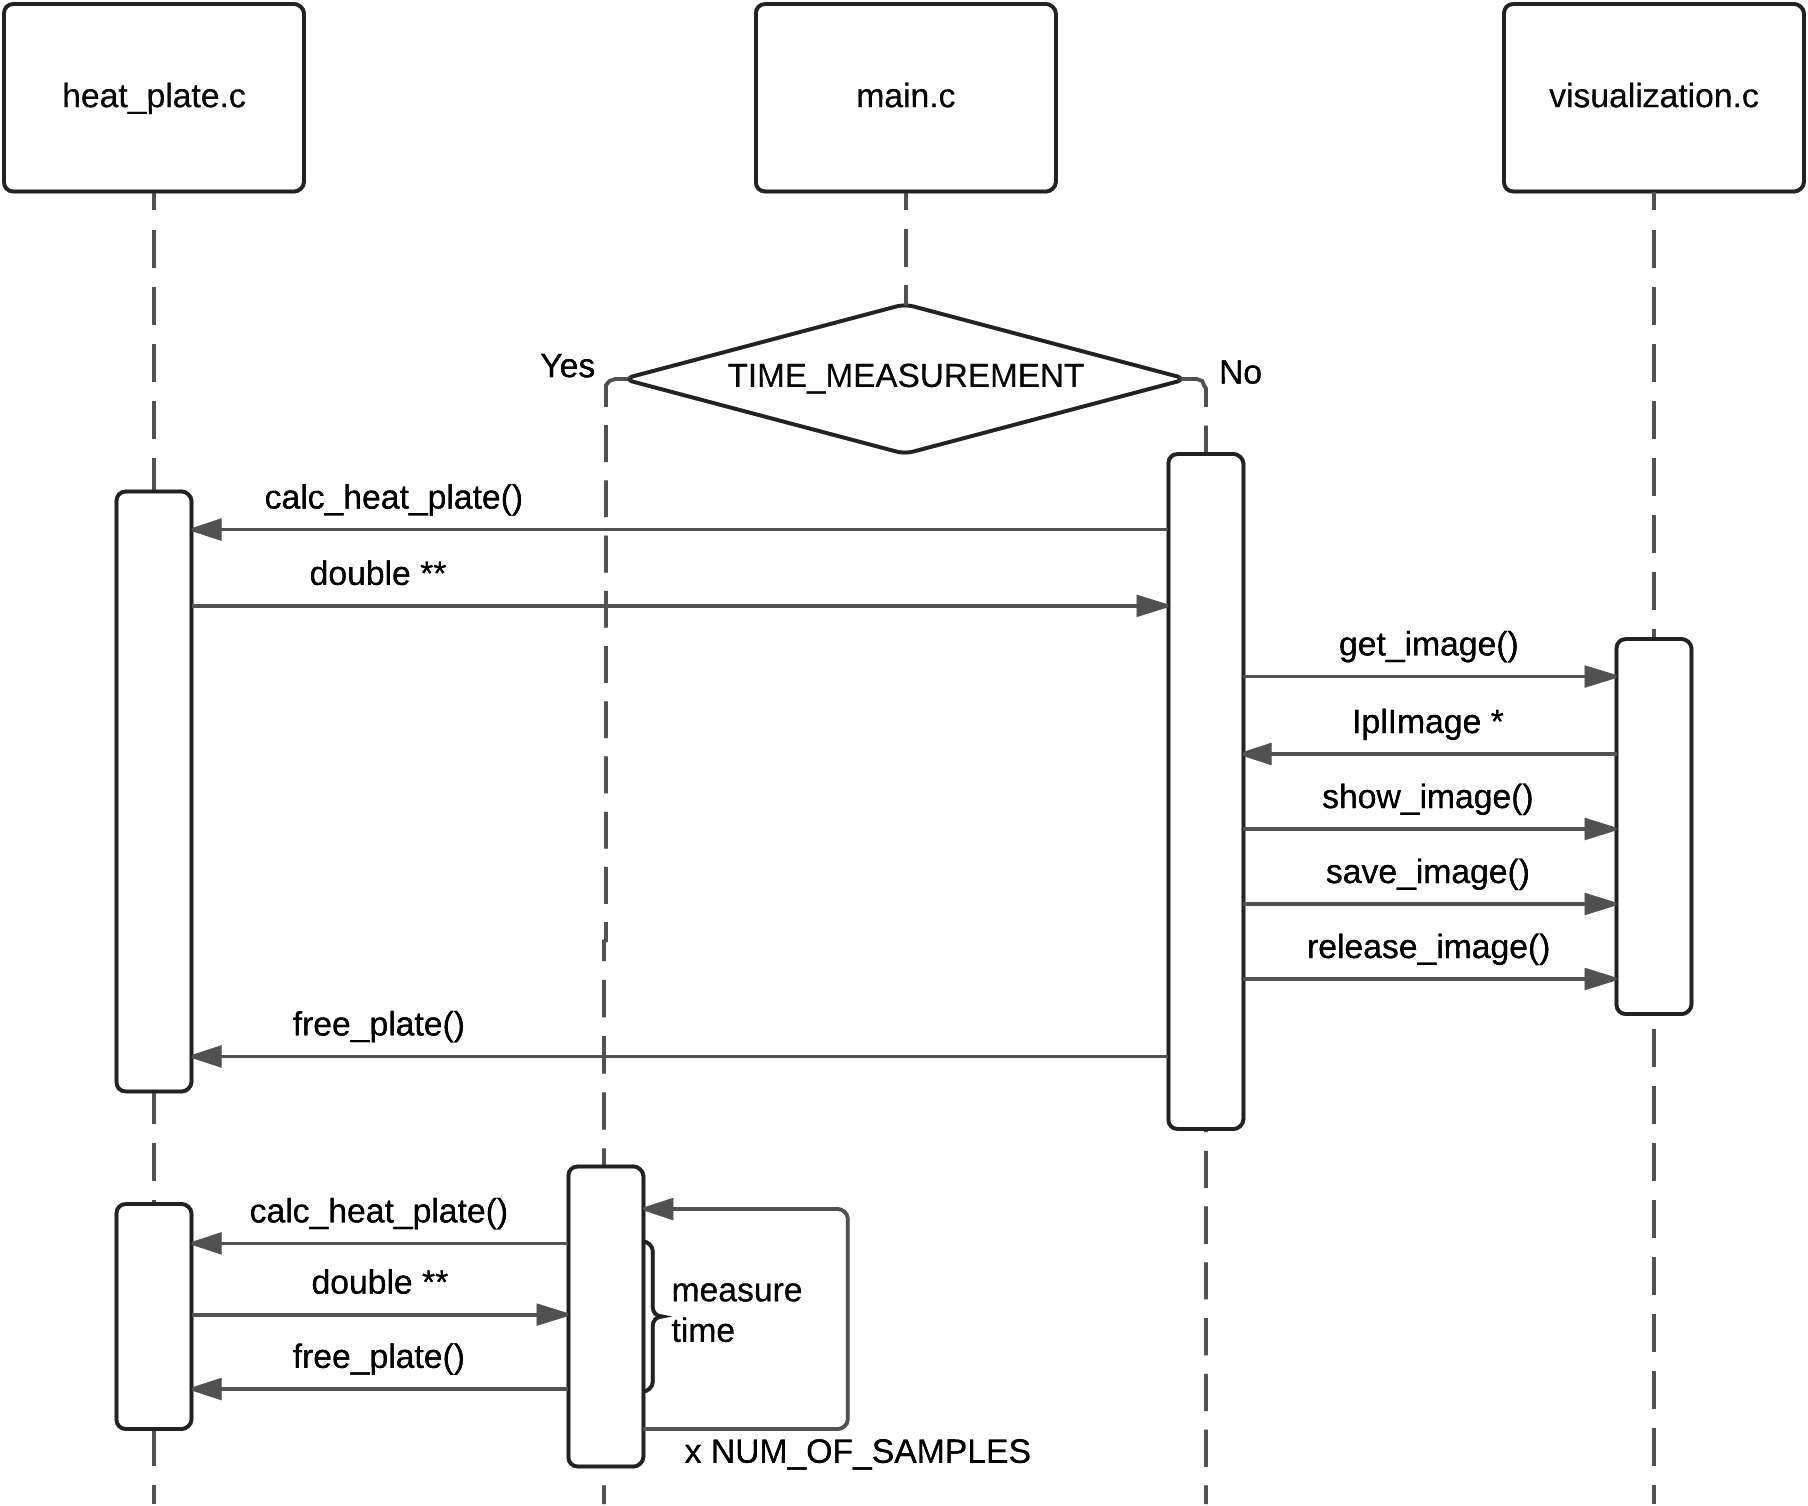
\includegraphics[scale=0.8]{diagram-zaporedja.png}
\caption{Diagram zaporedja, ki prikazuje delovanje programa.}
\label{diagram-zaporedja}
\end{center}
\vspace{-25pt}
\end{figure}

\subsection{Uporabljene knjižnice} \label{section-uporabljene-knjiznice}

Za vizualizacijo temperaturne plošče uporabljava knjižnico \textit{OpenCV}. Najprej se pripravi prazna slika (\textit{cvCreateImage}) z dimenzijami naše plošče, nato pa se za vsako točko na plošči pretvori temperaturo v 3 8-bitne kanale (rdeča, zelena, modra) in vrednosti prepiše na sliko. Če slika z največjo stranico presega \textit{MAX\_SIZE}, potem se jo še pomanjša (\textit{cvResize}). Pripravljeno sliko se prikaže (\textit{cvShowImage}) v oknu (\textit{cvNamedWindow}, \textit{cvMoveWindow}, \textit{cvResizeWindow}) in shrani na disk (\textit{cvSaveImage}). Na koncu se le še sprosti zaseden pomnilnik (\textit{cvReleaseImage}). Primer vizualizacije je viden na sliki \ref{primer-temperaturne-plosce}.

\section{Rezultati}

Program je bil testiran na sistemu, katerega specifikacije so navedene v tabeli \ref{tabela-specifikacije}. Da bi k izmerjenemu času čim manj pripomogli stroški režije operacijskega sistema, je bil sistem med testiranjem minimalno obremenjen z drugimi procesi.
\begin{table}[H]
\begin{center}
\caption{Specifikacije testnega sistema.}
\label{tabela-specifikacije}
\begin{tabularx}{\textwidth}{|YY|}
\hhline{==}
Procesor: & Intel Core i5-4210U\tabularnewline
Frekvenca procesorja: & 1.70GHz \tabularnewline
Število jeder: & 2 \tabularnewline
Maksimalno število niti: & 4 \tabularnewline
Velikost predpomnilnika: & 3MB \tabularnewline
Velikost in tip glavnega pomnilnika: & 16GB DDR3 \tabularnewline
Grafična kartica: & NVIDIA GeForce 820M 2GB DDR3 \tabularnewline
Operacijski sistem: & Ubuntu 16.04 \tabularnewline
\hhline{==}
\end{tabularx}
\end{center}
\vspace{-25pt}
\end{table}

Pri testiranju sva se omejila na fiksno velikost temperaturne plošče ($500 \times 500$) in spreminjala zgolj število iteracij. Za vsako izbrano število iteracij sva program 100-krat zagnala in vsakič izmerila čas izvajanja. Iz meritev sva nato izračunala povprečni čas izvajanja in standardno napako meritve, ki predstavlja razpršenost meritev okoli povprečnega časa izvajanja. Rezultati so navedeni tabelarično v tabeli \ref{tabela-rezultati-sekvencni} in z grafom, prikazanim na sliki \ref{graf-rezultati-1}.

\begin{table}[H]
\begin{center}
\caption{Povprečni čas izvajanja programa in standardna napaka meritev v odvisnosti od števila iteracij.}
\label{tabela-rezultati-sekvencni}
\begin{tabularx}{\textwidth}{|YYY|}
\hhline{===}
Število iteracij & Povprečni čas izvajanja [s] & Standardna napaka [s] \tabularnewline
\hhline{===}
500 & 1,698 & 0,001 \tabularnewline
1000 & 3,400 & 0,003 \tabularnewline
2000 & 6,780 & 0,003 \tabularnewline
5000 & 17,757 & 0,103 \tabularnewline
10000 & 33,972 & 0,026 \tabularnewline
20000 & 67,940 & 0,024 \tabularnewline
\hhline{===}
\end{tabularx}
\end{center}
\vspace{-25pt}
\end{table}

\begin{figure}[H]
\begin{center}
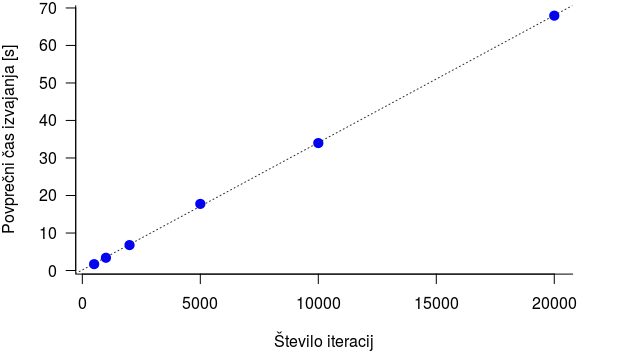
\includegraphics[scale=0.8]{graf-rezultati-1.png}
\caption{Graf, ki prikazuje povprečni čas izvajanja programa v odvisnosti od števila iteracij.}
\label{graf-rezultati-1}
\end{center}
\vspace{-25pt}
\end{figure}

Iz rezultatov je vidno, da je povprečni čas izvajanja linearno odvisen od števila iteracij, kar ustreza tudi teoretični časovni zahtevnosti \(O(k \cdot h \cdot w)\), kjer je \textit{k} število iteracij, \textit{h} višina, \textit{w} pa širina plošče. Točke na grafu se zelo lepo prilegajo funkciji \(t(k) = 0.003393 \cdot k + 0.150600\), iz te pa lahko razberemo, da algoritem na testnem sistemu potrebuje približno 0.003393 s za posamezno iteracijo (za \(h=w=500\)), 0.150600 s pa se porabi za ostale operacije, ki niso odvisne od števila iteracij.

\end{document}
